%!TEX root = ../thesis.tex

\section{実験概要}
%\begin{figure}[hbtp]
  %\centering
 %\includegraphics[keepaspectratio, scale=0.8]
      %{images/RaspberryPiMouse.png}
 %\caption{Example}
 %\label{Fig:Example}
%\end{figure}
%\subsection{実験概要}
本研究では,本研究室で開発されているロボット ORNE-box3\cite{井口颯人2023屋外自律移動ロボットプラットフォーム-orne} を用いて走行実験を行った.実機ロボットの外観は\figref{Fig:ORNE-box3}に示す.ORNE-box3のセンサ構成については、\figref{Fig:sensor configuration}に示すように,PCとしてJetson Orin NX 16GBを搭載しており、3D LiDAR:R-Fans-16
、IMU:ADIS16465、Encoder : i-Cart middleを備えている.3D LiDARは、自己位置推定と障害物検知に使用し、IMUとエンコーダは、emcl2に対して情報を提供している.

走行ルートは\figref{Fig:Course map of the Tsudanuma Challenge 2025}が示すように,津田沼校舎2号館前から食堂前に設置されたコーンまでとし,
津田沼チャレンジのコースの一部を利用した.このルートは,屋外環境における
自律移動性能を評価するための実環境を想定したものである.


実験では,Navigation2 における各種パラメータを個別に変化させた場合の
ロボットの挙動の変化を調査することを目的とした.
各走行実験においては,対象とするパラメータのみを変更し,
それ以外のパラメータはすべて一定に保った.

また,パラメータの変更に際しては,変更前の設定値を基準値とし,
基準値から増減させた場合のロボットの走行挙動を比較・分析した.
これにより,各パラメータがロボットの走行安定性や挙動に与える影響を
明確にすることを試みた.

\begin{figure}[hbtp]
  \centering
 \includegraphics[keepaspectratio, scale=0.6]
      {images/tsudanumachallenge.png}
 \caption{Course map of the Tsudanuma Challenge 2025(source: \cite{Tsudanumachallenge})}
 \label{Fig:Course map of the Tsudanuma Challenge 2025}
\end{figure}

\begin{figure}[hbtp]
  \centering
 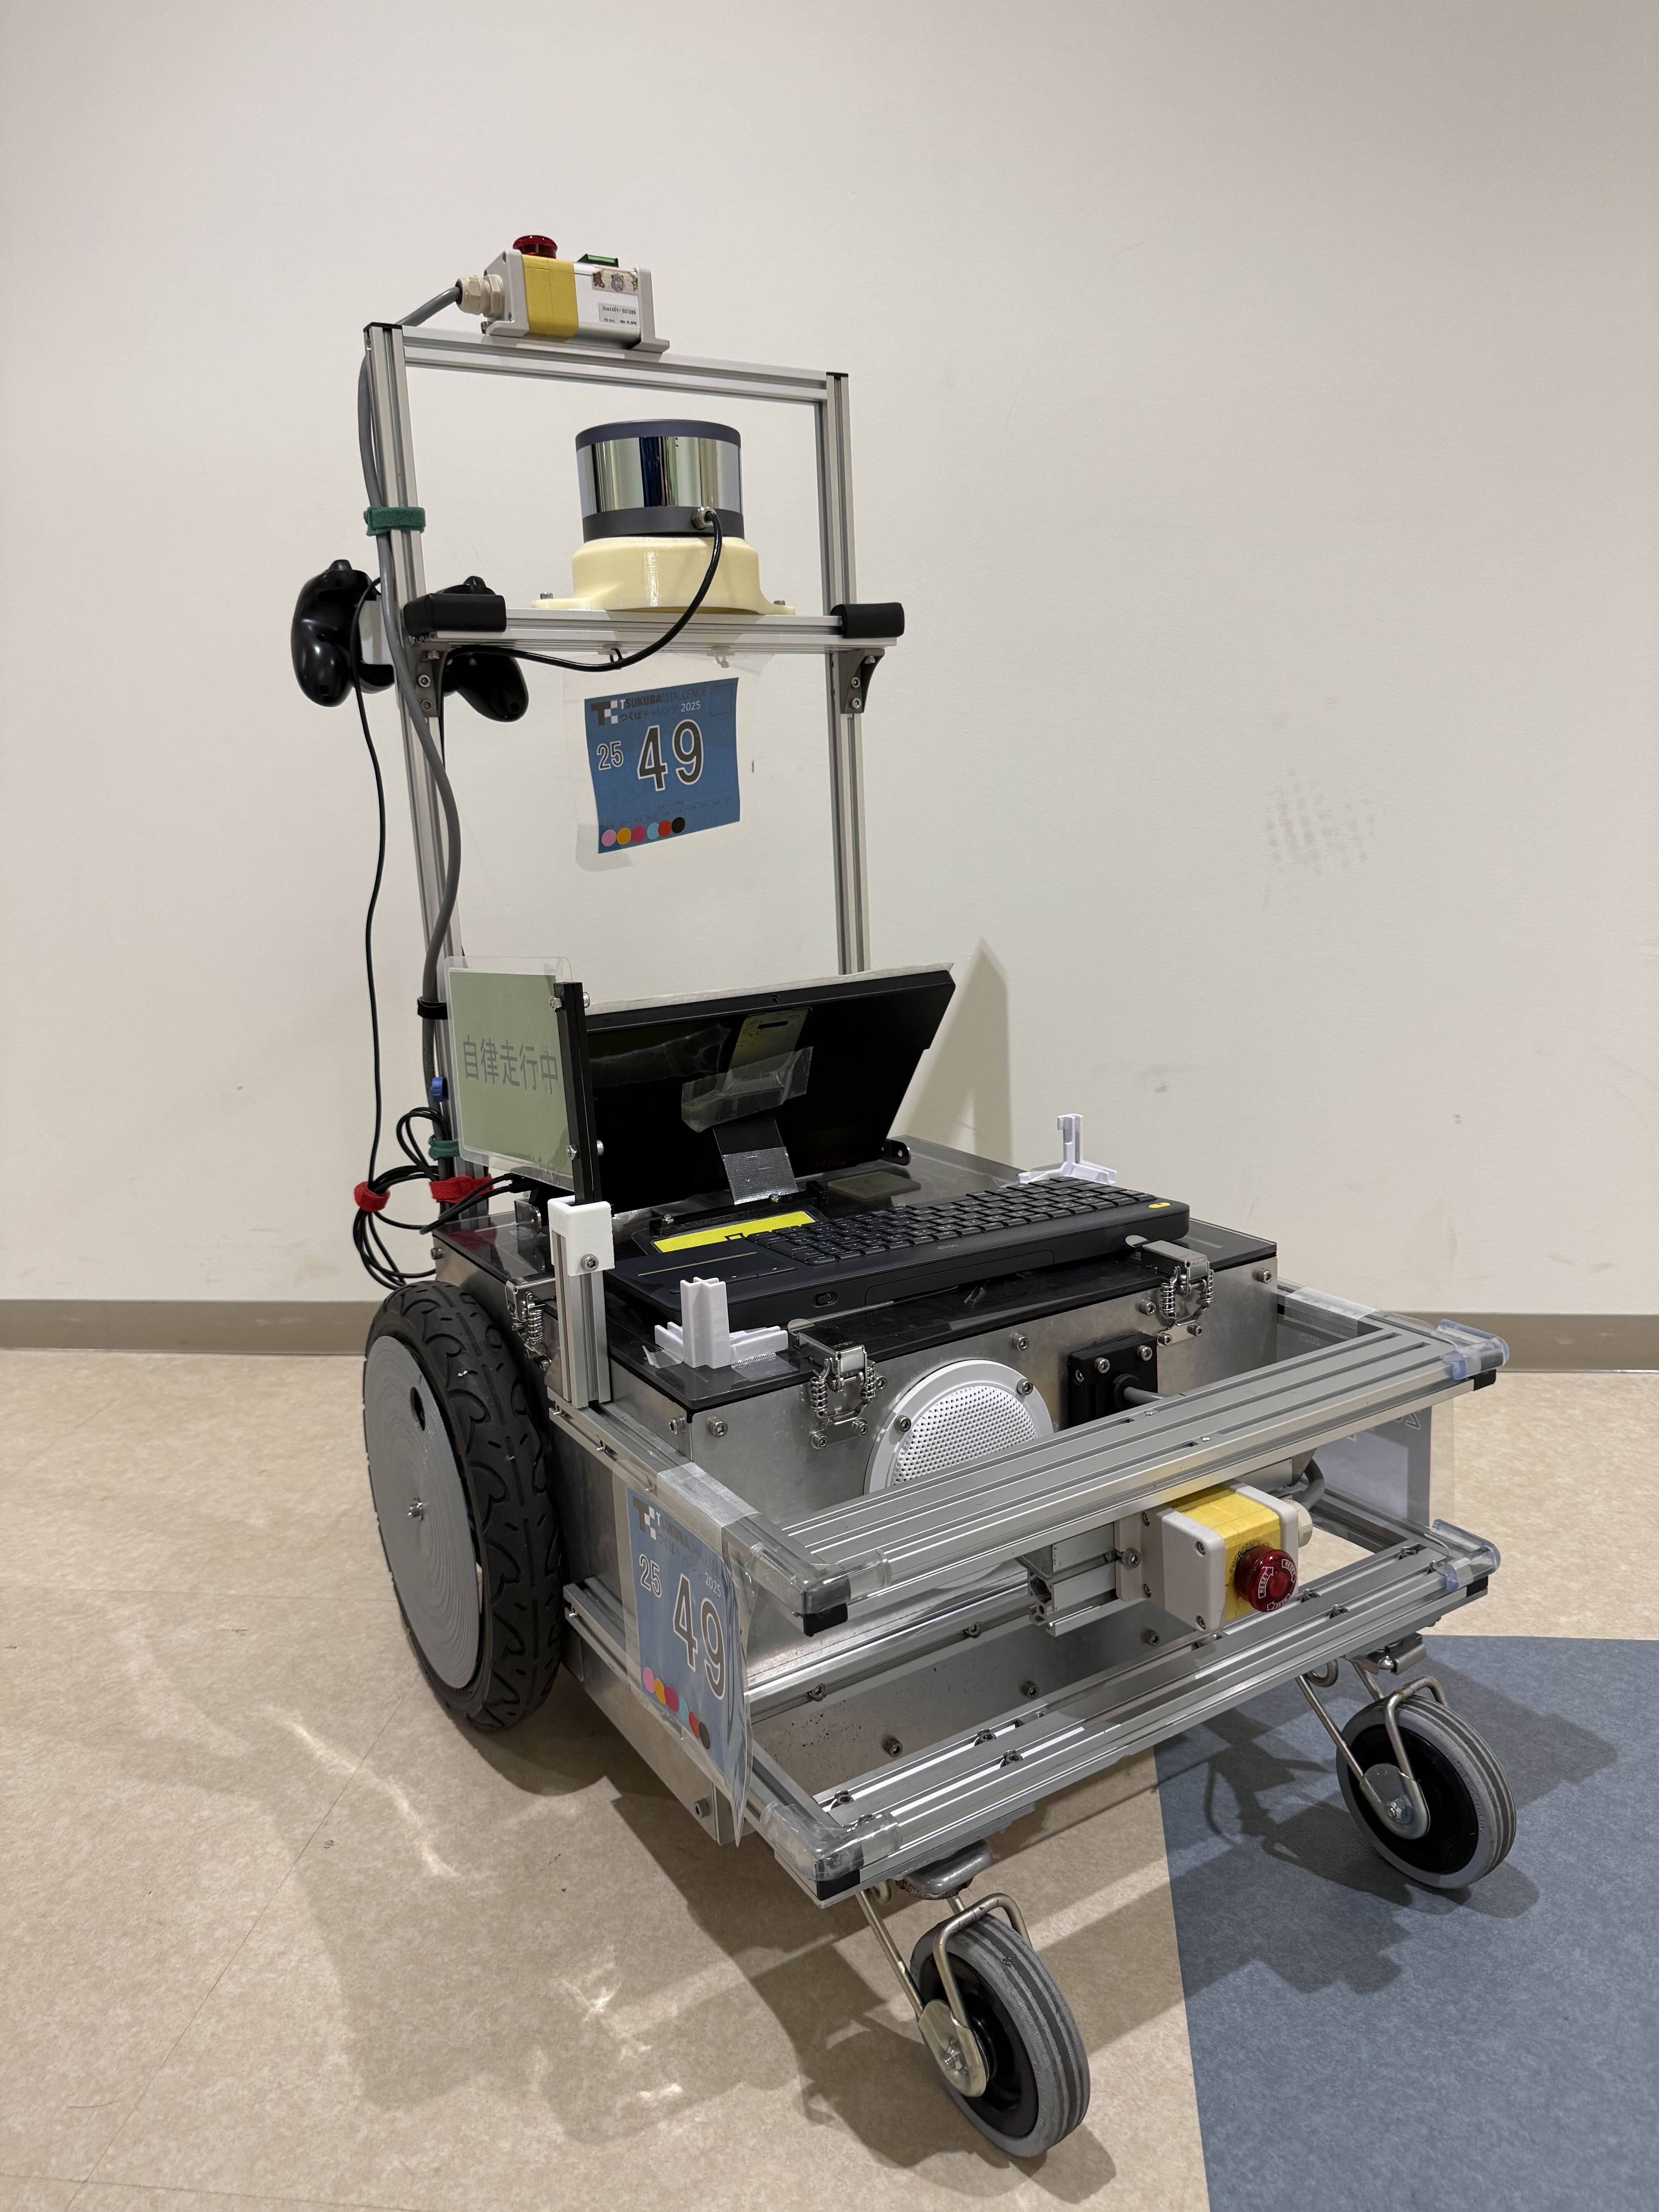
\includegraphics[keepaspectratio, scale=0.3]
      {images/orne-box3.png}
 \caption{ORNE-box3(source: \cite{井口颯人2023屋外自律移動ロボットプラットフォーム-orne})}
 \label{Fig:ORNE-box3}
\end{figure}
\begin{figure}[hbtp]
  \centering
 \includegraphics[keepaspectratio, scale=0.3]
      {images/sensor.png}
 \caption{sensor configuration}
 \label{Fig:sensor configuration}
\end{figure}
%\subsubsection{etc...}






\newpage

\section{実験結果}
%\begin{figure}[hbtp]
  %\centering
 %\includegraphics[keepaspectratio, scale=0.8]
      %{images/RaspberryPiMouse.png}
 %\caption{Example}
 %\label{Fig:Example}
%\end{figure}
\subsection{実験結果(emcl2)}
\subsubsection{実験結果(num\_particles)}

\begin{table}[H]
  \centering
  \caption{パーティクル数の違いによるゴール到達可否}
  \label{tab:num_particles_result}
  \begin{tabular}{c|c|c|c}
    \hline
    & \multicolumn{3}{c}{Number of particles} \\
    \hline
    number of times  & 200 & 500 (base) & 1000 \\
    \hline
    1  & $\times$ & ○ & ○ \\
    2  & ○ & ○ & $\times$ \\
    3  & $\times$ & $\times$ & $\times$ \\
    4  & ○ & ○ & ○ \\
    5  & ○ & ○ & $\times$ \\
    6  & $\times$ & $\times$ & $\times$ \\
    7  & ○ & ○ & ○ \\
    8  & ○ & ○ & ○ \\
    9  & ○ & ○ & ○ \\
    10 & ○ & ○ & ○ \\
    \hline
  \end{tabular}
\end{table}

Table\ref{tab:num_particles_result}に、パーティクル数の違いによるゴール到達の可否を示す.

\begin{table}[H]
  \centering
  \caption{パーティクル数ごとのゴール到達成功率}
  \label{tab:num_particles_success_rate}
  \begin{tabular}{c|c}
    \hline
    パーティクル数 & 成功率 [\%] \\
    \hline
    200  & 60 \\
    500 (base) & 80 \\
    1000 & 60 \\
    \hline
  \end{tabular}
\end{table}

Table\ref{tab:num_particles_success_rate}に,
パーティクル数を変化させた際のゴール到達成功率を示す.

Table\ref{tab:num_particles_result},Table\ref{tab:num_particles_success_rate}が示すように、パーティクル数を 200,500,1000 と変化させて自己位置推定の安定性を評価した.
その結果,パーティクル数 500 の場合に最も高いゴール到達率が得られた.
一方で,200 および 1000 の場合は,到達率がやや低下する傾向が確認された.
パーティクル数が少ないと自己位置推定が破綻しやすく、成功率が低下した.また、パーティクル数が多すぎても計算量の増加によって、遅延が発生して安定性が低下した。
以上より,パーティクル数は多ければ良いわけではなく,
自己位置推定の精度と計算負荷のバランスを考慮した適切な設定が重要であることが分かる.
本実験環境においては,パーティクル数 500 が最も安定した性能を示した.

次からの実験では、\figref{Fig:base orientation},\figref{Fig:base position}のグラフが基準の値の時のロボットの挙動である。\figref{Fig:base orientation}はロボットの向き、\figref{Fig:base position}はロボットの位置のグラフである。
\begin{figure}[H]
  \centering
 \includegraphics[keepaspectratio, scale=0.65]
      {images/base_muki2.png}
 \caption{base orientation}
 \label{Fig:base orientation}
\end{figure}
\begin{figure}[H]
  \centering
 \includegraphics[keepaspectratio, scale=0.5]
      {images/base_postion.png}
 \caption{base position}
 \label{Fig:base position}
\end{figure}

\subsubsection{実験結果(odom\_fw\_dev\_per\_fw)}
\figref{Fig:base orientation},\figref{Fig:base position}で示すように基準の値は、0.19
\begin{figure}[H]
  \centering
 \includegraphics[keepaspectratio, scale=0.6]
      {images/fwfw0.01muki.png}
 \caption{Robot orientation with fw\_dev\_per\_fw = 0.01}
 \label{Fig:Robot orientation with fw_dev_per_fw = 0.01 }
\end{figure}
\begin{figure}[H]
  \centering
 \includegraphics[keepaspectratio, scale=0.6]
      {images/fwfw0.01iti.png}
 \caption{Robot position with fw\_dev\_per\_fw = 0.01
}
 \label{Fig:Robot position with fw_dev_per_fw = 0.01}
\end{figure}

\begin{figure}[H]
  \centering
 \includegraphics[keepaspectratio, scale=0.6]
      {images/fwfw0.05muki2.png}
 \caption{Robot orientation with fw\_dev\_per\_fw = 0.05}
 \label{Fig:Robot orientation with fw_dev_per_fw = 0.05 }
\end{figure}
\begin{figure}[H]
  \centering
 \includegraphics[keepaspectratio, scale=0.6]
      {images/fwfw0.05iti2.png}
 \caption{Robot position with fw\_dev\_per\_fw = 0.05
}
 \label{Fig:Robot position with fw_dev_per_fw = 0.05}
\end{figure}

\begin{figure}[H]
  \centering
 \includegraphics[keepaspectratio, scale=0.6]
      {images/fwfw0.1muki2.png}
 \caption{Robot orientation with fw\_dev\_per\_fw = 0.1}
 \label{Fig:Robot orientation with fw_dev_per_fw = 0.1 }
\end{figure}
\begin{figure}[H]
  \centering
 \includegraphics[keepaspectratio, scale=0.6]
      {images/fwfw0.1iti2.png}
 \caption{Robot position with fw\_dev\_per\_fw = 0.1
}
 \label{Fig:Robot position with fw_dev_per_fw = 0.1}
\end{figure}

\begin{figure}[H]
  \centering
 \includegraphics[keepaspectratio, scale=0.6]
      {images/fwfw0.3muki.png}
 \caption{Robot orientation with fw\_dev\_per\_fw = 0.3}
 \label{Fig:Robot orientation with fw_dev_per_fw = 0.3 }
\end{figure}
\begin{figure}[H]
  \centering
 \includegraphics[keepaspectratio, scale=0.6]
      {images/fwfw0.3iti.png}
 \caption{Robot position with fw\_dev\_per\_fw = 0.3
}
 \label{Fig:Robot position with fw_dev_per_fw = 0.3}
\end{figure}

\begin{figure}[H]
  \centering
 \includegraphics[keepaspectratio, scale=0.6]
      {images/fwfw0.4muki.png}
 \caption{Robot orientation with fw\_dev\_per\_fw = 0.4}
 \label{Fig:Robot orientation with fw_dev_per_fw = 0.4 }
\end{figure}
\begin{figure}[H]
  \centering
 \includegraphics[keepaspectratio, scale=0.6]
      {images/fwfw0.4iti.png}
 \caption{Robot position with fw\_dev\_per\_fw = 0.4
}
 \label{Fig:Robot position with fw_dev_per_fw = 0.4}
\end{figure}

\begin{figure}[H]
  \centering
 \includegraphics[keepaspectratio, scale=0.6]
      {images/fwfw0.5muki.png}
 \caption{Robot orientation with fw\_dev\_per\_fw = 0.5}
 \label{Fig:Robot orientation with fw_dev_per_fw = 0.5 }
\end{figure}
\begin{figure}[H]
  \centering
 \includegraphics[keepaspectratio, scale=0.6]
      {images/fwfw0.5iti.png}
 \caption{Robot position with fw\_dev\_per\_fw = 0.5
}
 \label{Fig:Robot position with fw_dev_per_fw = 0.5}
\end{figure}

\figref{Fig:Robot orientation with fw_dev_per_fw = 0.5 }で示すように、odom\_fw\_dev\_per\_fw を 0.5 に設定した場合,ロボットは走行を続けるにつれて自己位置推定の誤差が累積し,最終的にゴールに到達することができなかった.一方で,0.4 以下の値に設定した場合には,ロボットはゴールまで到達することが確認された.

また,直線走行時の挙動を基準条件と比較すると,odom\_fw\_dev\_per\_fw を大きく設定した場合には,推定されたロボットの位置が徐々にずれていく様子が確認された.このことから,odom\_fw\_dev\_per\_fw の値を過度に大きくすると,前進移動に対するオドメトリ誤差が強調され,自己位置推定の精度が低下することが示唆される.

%\figref{Fig:Robot orientation with fw_dev_per_fw = 0.01 },\figref{Fig:Robot position with fw_dev_per_fw = 0.01}

\subsubsection{実験結果(odom\_fw\_dev\_per\_rot)}
\figref{Fig:base orientation},\figref{Fig:base position}で示すように、基準の値は、0.0001

\begin{figure}[H]
  \centering
 \includegraphics[keepaspectratio, scale=0.6]
      {images/fwrot0.001muki.png}
 \caption{Robot orientation with fw\_dev\_per\_rot = 0.001}
 \label{Fig:Robot orientation with fw_dev_per_rot = 0.001 }
\end{figure}
\begin{figure}[H]
  \centering
 \includegraphics[keepaspectratio, scale=0.6]
      {images/fwrot0.001iti.png}
 \caption{Robot position with fw\_dev\_per\_rot = 0.001
}
 \label{Fig:Robot position with fw_dev_per_rot = 0.001}
\end{figure}

\begin{figure}[H]
  \centering
 \includegraphics[keepaspectratio, scale=0.6]
      {images/fwrot0.01muki.png}
 \caption{Robot orientation with fw\_dev\_per\_rot = 0.01}
 \label{Fig:Robot orientation with fw_dev_per_rot = 0.01 }
\end{figure}
\begin{figure}[H]
  \centering
 \includegraphics[keepaspectratio, scale=0.6]
      {images/fwrot0.01iti.png}
 \caption{Robot position with fw\_dev\_per\_rot = 0.01
}
 \label{Fig:Robot position with fw_dev_per_rot = 0.01}
\end{figure}

\begin{figure}[H]
  \centering
 \includegraphics[keepaspectratio, scale=0.6]
      {images/fwrot0.1muki.png}
 \caption{Robot orientation with fw\_dev\_per\_rot = 0.1}
 \label{Fig:Robot orientation with fw_dev_per_rot = 0.1 }
\end{figure}
\begin{figure}[H]
  \centering
 \includegraphics[keepaspectratio, scale=0.6]
      {images/fwrot0.1iti.png}
 \caption{Robot position with fw\_dev\_per\_rot = 0.1
}
 \label{Fig:Robot position with fw_dev_per_rot = 0.1}
\end{figure}

\begin{figure}[H]
  \centering
 \includegraphics[keepaspectratio, scale=0.6]
      {images/fwrot0.5muki.png}
 \caption{Robot orientation with fw\_dev\_per\_rot = 0.5}
 \label{Fig:Robot orientation with fw_dev_per_rot = 0.5 }
\end{figure}
\begin{figure}[H]
  \centering
 \includegraphics[keepaspectratio, scale=0.6]
      {images/fwrot0.5iti.png}
 \caption{Robot position with fw\_dev\_per\_rot = 0.5
}
 \label{Fig:Robot position with fw_dev_per_rot = 0.5}
\end{figure}

odom\_fw\_dev\_per\_rot を変化させた実験では,すべての設定値においてロボットはゴールに到達することができた.特に,odom\_fw\_dev\_per\_rot を 0.5 に設定した場合には,走行中に自己位置推定のずれが一部確認されたものの,走行不能となるような大きな影響は見られず,最終的にゴールまで到達することが確認された.

この結果から,odom\_fw\_dev\_per\_rot は自己位置推定に一定の影響を与えるものの,fw 方向の移動誤差を表す odom\_fw\_dev\_per\_fw と比較すると,ゴール到達性に与える影響は相対的に小さいと考えられる.


\subsubsection{実験結果(odom\_rot\_dev\_per\_fw)}
\figref{Fig:base orientation},\figref{Fig:base position}で示すように基準の値は、0.13

\begin{figure}[H]
  \centering
 \includegraphics[keepaspectratio, scale=0.6]
      {images/rotfw0.01muki.png}
 \caption{Robot orientation with rot\_dev\_per\_fw = 0.01}
 \label{Fig:Robot orientation with rot_dev_per_fw = 0.01 }
\end{figure}
\begin{figure}[H]
  \centering
 \includegraphics[keepaspectratio, scale=0.6]
      {images/rotfw0.01iti.png}
 \caption{Robot position with rot\_dev\_per\_fw = 0.01
}
 \label{Fig:Robot position with rot_dev_per_fw = 0.01}
\end{figure}

\begin{figure}[H]
  \centering
 \includegraphics[keepaspectratio, scale=0.6]
      {images/rotfw0.2muki.png}
 \caption{Robot orientation with rot\_dev\_per\_fw = 0.2}
 \label{Fig:Robot orientation with rot_dev_per_fw = 0.2 }
\end{figure}
\begin{figure}[H]
  \centering
 \includegraphics[keepaspectratio, scale=0.6]
      {images/rotfw0.2iti.png}
 \caption{Robot position with rot\_dev\_per\_fw = 0.2
}
 \label{Fig:Robot position with rot_dev_per_fw = 0.2}
\end{figure}

\begin{figure}[H]
  \centering
 \includegraphics[keepaspectratio, scale=0.6]
      {images/rotfw0.3muki.png}
 \caption{Robot orientation with rot\_dev\_per\_fw = 0.3}
 \label{Fig:Robot orientation with rot_dev_per_fw = 0.3 }
\end{figure}
\begin{figure}[H]
  \centering
 \includegraphics[keepaspectratio, scale=0.6]
      {images/rotfw0.3iti.png}
 \caption{Robot position with rot\_dev\_per\_fw = 0.3
}
 \label{Fig:Robot position with rot_dev_per_fw = 0.3}
\end{figure}

\begin{figure}[H]
  \centering
 \includegraphics[keepaspectratio, scale=0.6]
      {images/rotfw0.4muki.png}
 \caption{Robot orientation with rot\_dev\_per\_fw = 0.4}
 \label{Fig:Robot orientation with rot_dev_per_fw = 0.4 }
\end{figure}
\begin{figure}[H]
  \centering
 \includegraphics[keepaspectratio, scale=0.6]
      {images/rotfw0.4iti.png}
 \caption{Robot position with rot\_dev\_per\_fw = 0.4
}
 \label{Fig:Robot position with rot_dev_per_fw = 0.4}
\end{figure}

\begin{figure}[H]
  \centering
 \includegraphics[keepaspectratio, scale=0.6]
      {images/rotfw0.5muki.png}
 \caption{Robot orientation with rot\_dev\_per\_fw = 0.5}
 \label{Fig:Robot orientation with rot_dev_per_fw = 0.5 }
\end{figure}
\begin{figure}[H]
  \centering
 \includegraphics[keepaspectratio, scale=0.6]
      {images/rotfw0.5iti.png}
 \caption{Robot position with rot\_dev\_per\_fw = 0.5
}
 \label{Fig:Robot position with rot_dev_per_fw = 0.5}
\end{figure}

rot\_dev\_per\_fwでの実験では、rot\_dev\_per\_fw の値を大きくした場合においても,ロボットは直進走行中に自己位置および姿勢のわずかなずれが生じるのみであり,走行不能となることはなく,最終的にゴールまで問題なく到達することが確認された.

直線走行区間(目標方位 270°)でのロボットの向きに着目すると,rot\_dev\_per\_fw を 0.01 に設定した\figref{Fig:Robot orientation with rot_dev_per_fw = 0.01 }の場合には,ロボットは目標方位をほぼ維持したまま高い精度で直進していることが確認できた.一方で,rot\_dev\_per\_fw を 0.4 以上に設定した\figref{Fig:Robot orientation with rot_dev_per_fw = 0.4 },\figref{Fig:Robot orientation with rot_dev_per_fw = 0.5 }で示した場合には,走行中のロボットの方位が 270° を下回る傾向が見られ,進行に伴って姿勢が徐々にずれていく様子が確認された.

しかしながら,この方位のずれはナビゲーション全体に致命的な影響を与えるほどではなく,ゴール到達性に大きな影響は見られなかった.


\subsubsection{実験結果(odom\_rot\_dev\_per\_rot)}
\figref{Fig:base orientation},\figref{Fig:base position}で示すように基準の値は、0.19

\begin{figure}[H]
  \centering
 \includegraphics[keepaspectratio, scale=0.6]
      {images/rotrot0.1muki2.png}
 \caption{Robot orientation with rot\_dev\_per\_rot = 0.1}
 \label{Fig:Robot orientation with rot_dev_per_rot = 0.1 }
\end{figure}
\begin{figure}[H]
  \centering
 \includegraphics[keepaspectratio, scale=0.6]
      {images/rotrot0.1iti.png}
 \caption{Robot position with rot\_dev\_per\_rot = 0.1
}
 \label{Fig:Robot position with rot_dev_per_rot = 0.1}
\end{figure}

\begin{figure}[H]
  \centering
 \includegraphics[keepaspectratio, scale=0.6]
      {images/rotrot0.3muki.png}
 \caption{Robot orientation with rot\_dev\_per\_rot = 0.3}
 \label{Fig:Robot orientation with rot_dev_per_rot = 0.3 }
\end{figure}
\begin{figure}[H]
  \centering
 \includegraphics[keepaspectratio, scale=0.6]
      {images/rotrot0.3iti.png}
 \caption{Robot position with rot\_dev\_per\_rot = 0.3
}
 \label{Fig:Robot position with rot_dev_per_rot = 0.3}
\end{figure}

\begin{figure}[H]
  \centering
 \includegraphics[keepaspectratio, scale=0.6]
      {images/rotrot0.4muki.png}
 \caption{Robot orientation with rot\_dev\_per\_rot = 0.4}
 \label{Fig:Robot orientation with rot_dev_per_rot = 0.4 }
\end{figure}
\begin{figure}[H]
  \centering
 \includegraphics[keepaspectratio, scale=0.6]
      {images/rotrot0.4iti.png}
 \caption{Robot position with rot\_dev\_per\_rot = 0.4
}
 \label{Fig:Robot position with rot_dev_per_rot = 0.4}
\end{figure}

\begin{figure}[H]
  \centering
 \includegraphics[keepaspectratio, scale=0.6]
      {images/rotrot0.5muki.png}
 \caption{Robot orientation with rot\_dev\_per\_rot = 0.5}
 \label{Fig:Robot orientation with rot_dev_per_rot = 0.5 }
\end{figure}
\begin{figure}[H]
  \centering
 \includegraphics[keepaspectratio, scale=0.6]
      {images/rotrot0.5iti.png}
 \caption{Robot position with rot\_dev\_per\_rot = 0.5
}
 \label{Fig:Robot position with rot_dev_per_rot = 0.5}
\end{figure}

%\subsection{rot\_dev\_per\_rot に関する実験結果}
rot\_dev\_per\_rot は,emcl において回転量に比例して付加される回転誤差を表すパラメータであり,
値が大きいほどセンサ情報を重視し,値が小さいほどオドメトリ情報を重視する設定となる.

本実験の結果,rot\_dev\_per\_rot の値を大きく設定した場合,
自己位置推定においてセンサの影響が強くなり,
ロボットの姿勢推定が不安定となることで,走行中の挙動がふらつく傾向が確認された.

特に旋回動作時においてセンサ重視の設定とした場合,
ゴール付近で自己位置推定が不安定となり,
rot\_dev\_per\_rot を 0.5 および 0.4 に設定した条件では,
ロボットがゴール端付近で停止し,正常にゴールへ到達できない事例が確認された.

以上より,rot\_dev\_per\_rot を過度に大きく設定すると,
回転時の姿勢推定においてセンサノイズの影響を受けやすくなり,
ナビゲーション性能が低下する可能性があることが示唆される.


\subsubsection{実験結果(laser\_likelihood\_max\_dist)}

\figref{Fig:base orientation},\figref{Fig:base position}で示すように基準の値は、0.2

\begin{figure}[H]
  \centering
 \includegraphics[keepaspectratio, scale=0.6]
      {images/llmd0.5muki.png}
 \caption{Robot orientation with laser\_likelihood\_max\_dist = 0.5}
 \label{Fig:Robot orientation with laser_likelihood_max_dist = 0.5 }
\end{figure}
\begin{figure}[H]
  \centering
 \includegraphics[keepaspectratio, scale=0.6]
      {images/llmd0.5iti.png}
 \caption{Robot position with laser\_likelihood\_max\_dist = 0.5
}
 \label{Fig:Robot position with laser_likelihood_max_dist = 0.5}
\end{figure}

\begin{figure}[H]
  \centering
 \includegraphics[keepaspectratio, scale=0.6]
      {images/llmd1.0muki.png}
 \caption{Robot orientation with laser\_likelihood\_max\_dist = 1.0}
 \label{Fig:Robot orientation with laser_likelihood_max_dist = 1.0 }
\end{figure}
\begin{figure}[H]
  \centering
 \includegraphics[keepaspectratio, scale=0.6]
      {images/llmd1.0iti.png}
 \caption{Robot position with laser\_likelihood\_max\_dist = 1.0
}
 \label{Fig:Robot position with laser_likelihood_max_dist = 1.0}
\end{figure}


本実験では,基準値から laser\_likelihood\_max\_dist の値を増加させた場合,
レーザによって評価される情報量が増加し,
特に障害物や構造物が多く存在する環境において,
自己位置推定の更新が頻繁に行われることが確認された.

その結果,レーザスキャンによる評価負荷が高い箇所では,
ロボットが一時的に停止する挙動が観測された.
これは,自己位置推定の更新に伴い,
ナビゲーションが安全側に制御されたためであると考えられる.

一方で,laser\_likelihood\_max\_dist を約 0.5 程度まで増加させた場合でも,
ロボットは全体として安定した走行が可能であり,
大きなナビゲーション性能の低下は確認されなかった.

\subsubsection{実験結果(range\_threshold)}

\figref{Fig:base orientation},\figref{Fig:base position}で示すように基準の値は、0.3
\begin{figure}[H]
  \centering
 \includegraphics[keepaspectratio, scale=0.6]
      {images/rt0.5muki.png}
 \caption{Robot orientation with range\_threshold = 0.5}
 \label{Fig:Robot orientation with range_threshold = 0.5 }
\end{figure}
\begin{figure}[H]
  \centering
 \includegraphics[keepaspectratio, scale=0.6]
      {images/rt0.5iti.png}
 \caption{Robot position with range\_threshold = 0.5
}
 \label{Fig:Robot position with range_threshold = 0.5}
\end{figure}

\begin{figure}[H]
  \centering
 \includegraphics[keepaspectratio, scale=0.6]
      {images/rt0.9muki.png}
 \caption{Robot orientation with range\_threshold = 0.9}
 \label{Fig:Robot orientation with range_threshold = 0.9 }
\end{figure}
\begin{figure}[H]
  \centering
 \includegraphics[keepaspectratio, scale=0.6]
      {images/rt0.9iti.png}
 \caption{Robot position with range\_threshold = 0.9
}
 \label{Fig:Robot position with range_threshold = 0.9}
\end{figure}

%\subsection{range\_threshold に関する実験結果}

本実験では、基準値である range\_threshold = 0.3 の場合,
ロボットは主に比較的近距離のレーザスキャン情報を用いて
自己位置推定を行っており,
推定された位置および姿勢は安定していた.

一方,range\_threshold を 0.9 に設定した場合,
より遠方のレーザスキャン情報も自己位置推定に使用されるため,
基準値の場合と比較して,
推定されたロボットの位置に明らかなずれが生じることや,
姿勢が異なる方向を示す場合が確認された.
しかしながら,これらのずれが生じた場合でも,
ロボットは最終的にゴール地点へ到達することができた.

また,range\_threshold を 0.5 に設定した場合には,
自己位置推定および走行挙動は安定しており,
基準値と比較して大きな性能低下は確認されなかった.

以上の結果より,range\_threshold は過度に大きな値を設定すると
自己位置推定の精度低下を招く可能性がある一方で,
0.5 程度までであれば,
安定したナビゲーションを維持したまま設定値を引き上げることが
可能であると考えられる.

以上の結果より,emcl2 における各パラメータは,
オドメトリ情報とレーザセンサ情報の信頼度のバランスを調整する役割を持ち,
設定値によって自己位置推定の特性および
ロボットの走行挙動が大きく変化することが明らかとなった.
そのため,実環境におけるナビゲーションでは,
各パラメータの意味を理解した上で,
環境特性に応じた適切な調整が重要であるといえる.

\subsection{実験結果(Nav2\_controller)}

\subsubsection{実験結果(max\_vel\_x)}
\figref{Fig:base orientation},\figref{Fig:base position}で示すように基準の値は、0.6

\begin{figure}[H]
  \centering
 \includegraphics[keepaspectratio, scale=0.6]
      {images/mvx0.2muki.png}
 \caption{Robot orientation with max\_vel\_x = 0.2}
 \label{Fig:Robot orientation with max_vel_x = 0.2 }
\end{figure}
\begin{figure}[H]
  \centering
 \includegraphics[keepaspectratio, scale=0.6]
      {images/mvx0.2iti.png}
 \caption{Robot position with max\_vel\_x = 0.2
}
 \label{Fig:Robot position with max_vel_x = 0.2}
\end{figure}


\begin{figure}[H]
  \centering
 \includegraphics[keepaspectratio, scale=0.6]
      {images/mvx1.0muki.png}
 \caption{Robot orientation with max\_vel\_x = 1.0}
 \label{Fig:Robot orientation with max_vel_x = 1.0 }
\end{figure}
\begin{figure}[H]
  \centering
 \includegraphics[keepaspectratio, scale=0.6]
      {images/mvx1.0iti.png}
 \caption{Robot position with max\_vel\_x = 1.0
}
 \label{Fig:Robot position with max_vel_x = 1.0}
\end{figure}

%\subsection{Controller における max\_vel\_x の実験結果}

%本実験では,Navigation2 の Controller における
%最大並進速度を制御するパラメータ max\_vel\_x を変更し,
%ロボットの走行挙動への影響を調査した.

まず,max\_vel\_x の値を小さく設定した場合,
ロボットの走行速度が低下し,
走行中の挙動が不安定になる傾向が確認された.
しかしながら,速度が低下した状態であっても,
ロボットはゴールまで到達することができ,
ナビゲーション自体が破綻することはなかった.

一方で,max\_vel\_x の値を基準値より大きく設定した場合,
走行挙動に大きな変化は見られず,
ロボットの実際の走行速度も基準値である 0.6\,[m/s] 以上には上昇しなかった.
この結果から,
max\_vel\_x を増加させても,
他のパラメータやシステム制約によって
ロボットの最大速度が制限されている可能性が考えられる.

以上のことから,
max\_vel\_x は走行速度の上限を設定する重要なパラメータである一方で,
ロボットの実際の最高速度は,
Controller 以外のパラメータや
ハードウェア設定の影響も受けることが示唆された.
この速度制限の要因については,
後述する実験において詳細に検証する.


\subsubsection{実験結果(max\_vel\_theta)}
\figref{Fig:base orientation},\figref{Fig:base position}で示すように基準の値は、0.7

\begin{figure}[H]
  \centering
 \includegraphics[keepaspectratio, scale=0.6]
      {images/mvt0.4muki.png}
 \caption{Robot orientation with max\_vel\_theta = 0.4}
 \label{Fig:Robot orientation with max_vel_theta = 0.4 }
\end{figure}
\begin{figure}[H]
  \centering
 \includegraphics[keepaspectratio, scale=0.6]
      {images/mvt0.4iti.png}
 \caption{Robot position with max\_vel\_theta = 0.4
}
 \label{Fig:Robot position with max_vel_theta = 0.4}
\end{figure}

\begin{figure}[H]
  \centering
 \includegraphics[keepaspectratio, scale=0.6]
      {images/mvt1.0muki.png}
 \caption{Robot orientation with max\_vel\_theta = 1.0}
 \label{Fig:Robot orientation with max_vel_theta = 1.0 }
\end{figure}
\begin{figure}[H]
  \centering
 \includegraphics[keepaspectratio, scale=0.6]
      {images/mvt1.0iti.png}
 \caption{Robot position with max\_vel\_theta = 1.0
}
 \label{Fig:Robot position with max_vel_theta = 1.0}
\end{figure}

%\subsection{Controller における max\_vel\_theta の実験結果}
%本実験では,Navigation2 の Controller における
%最大角速度を制御するパラメータ max\_vel\_theta を変更し,
%ロボットの旋回挙動への影響を調査した.

本実験で、max\_vel\_theta の値を基準値より大きく設定した場合,
ロボットの走行挙動に顕著な変化は見られなかった.
この結果から,
基準値の時点でロボットの旋回性能は十分に確保されており,
それ以上角速度の上限を引き上げても,
実際の挙動には大きく反映されないことが示唆される.

一方で,max\_vel\_theta の値を基準値より小さく設定した場合,
ロボットの挙動が不安定になる様子が確認された.
特に,旋回が必要となる箇所において,
ロボットが一時的に停止し,
旋回完了までに時間を要する場面が多く見られた.
さらに,旋回後の直進動作においても,
進行方向が安定せず,
ふらついた挙動を示す傾向が確認された.

以上の結果より,
max\_vel\_theta を過度に小さく設定すると,
旋回動作およびその後の直進動作に悪影響を及ぼし,
ナビゲーション全体の安定性が低下することが明らかとなった.
そのため,本パラメータは,
旋回性能を確保できる十分な値に設定することが重要である.


\subsubsection{実験結果(max\_speed\_xy)}
\figref{Fig:base orientation},\figref{Fig:base position}で示すように基準の値は、0.9

%0.1,0.5,1.5

\begin{figure}[H]
  \centering
 \includegraphics[keepaspectratio, scale=0.6]
      {images/msxy0.1muki.png}
 \caption{Robot orientation with max\_speed\_xy = 0.1}
 \label{Fig:Robot orientation with max_speed_xy = 0.1 }
\end{figure}
\begin{figure}[H]
  \centering
 \includegraphics[keepaspectratio, scale=0.6]
      {images/msxy0.1iti.png}
 \caption{Robot position with max\_speed\_xy = 0.1
}
 \label{Fig:Robot position with max_speed_xy = 0.1}
\end{figure}

\begin{figure}[H]
  \centering
 \includegraphics[keepaspectratio, scale=0.6]
      {images/msxy0.5muki.png}
 \caption{Robot orientation with max\_speed\_xy = 0.5}
 \label{Fig:Robot orientation with max_speed_xy = 0.5 }
\end{figure}
\begin{figure}[H]
  \centering
 \includegraphics[keepaspectratio, scale=0.6]
      {images/msxy0.5iti.png}
 \caption{Robot position with max\_speed\_xy = 0.5
}
 \label{Fig:Robot position with max_speed_xy = 0.5}
\end{figure}

\begin{figure}[H]
  \centering
 \includegraphics[keepaspectratio, scale=0.6]
      {images/msxy1.5muki.png}
 \caption{Robot orientation with max\_speed\_xy = 1.5}
 \label{Fig:Robot orientation with max_speed_xy = 1.5 }
\end{figure}
\begin{figure}[H]
  \centering
 \includegraphics[keepaspectratio, scale=0.6]
      {images/msxy1.5iti.png}
 \caption{Robot position with max\_speed\_xy = 1.5
}
 \label{Fig:Robot position with max_speed_xy = 1.5}
\end{figure}

%\subsection{Controller における max\_speed\_xy の実験結果}

%本実験では,Navigation2 の Controller において,
%並進方向の合成速度の上限を制御するパラメータ max\_speed\_xy を変更し,
%ロボットの走行挙動への影響を調査した.

本実験では、max\_speed\_xy を 0.5 に設定した場合,
ロボットは安定した走行を維持したままゴールへ到達することができた.
また,max\_speed\_xy を 1.5 に設定した場合においても,
ロボットの実際の走行速度に大きな変化は見られなかった.
この挙動は,
前節で述べた max\_vel\_x の実験結果と同様であり,
他のパラメータやシステム制約によって
ロボットの最大速度が制限されている可能性が考えられる.
この点については,後述する実験において検証を行う.

一方で,max\_speed\_xy を 0.1 に設定した場合,
ロボットの走行速度が極端に低下し,
ゴールまで到達することができなかった.
特に,走行開始後の初期段階において,
最初の曲がり角付近の段差に接触する挙動が確認された.
また,この設定値では,
曲がり角に進入する際に左右の車輪を交互に動かすような挙動が見られ,
滑らかな旋回動作が行われていなかった.

以上の結果より,
max\_speed\_xy を過度に小さく設定すると,
旋回動作が不安定となり,
ナビゲーションの遂行が困難になることが明らかとなった.
一方で,本パラメータを大きく設定した場合でも,
他の速度制限要因によって
実際の走行速度が制約される可能性があるため,
他の速度関連パラメータとの関係を考慮した調整が重要である.



\subsubsection{実験結果(min\_theta\_velocity\_threshold)}
\figref{Fig:base orientation},\figref{Fig:base position}で示すように基準の値は、0.001

0.01,0.1,1.0,
\begin{figure}[H]
  \centering
 \includegraphics[keepaspectratio, scale=0.6]
      {images/mtvt0.01muki.png}
 \caption{Robot orientation with min\_theta\_velocity\_threshold = 0.01}
 \label{Fig:Robot orientation with min_theta_velocity_threshold = 0.01 }
\end{figure}
\begin{figure}[H]
  \centering
 \includegraphics[keepaspectratio, scale=0.6]
      {images/mtvt0.01iti.png}
 \caption{Robot position with min\_theta\_velocity\_threshold = 0.01
}
 \label{Fig:Robot position with min_theta_velocity_threshold = 0.01}
\end{figure}
\begin{figure}[H]
  \centering
 \includegraphics[keepaspectratio, scale=0.6]
      {images/mtvt0.1muki.png}
 \caption{Robot orientation with min\_theta\_velocity\_threshold = 0.1}
 \label{Fig:Robot orientation with min_theta_velocity_threshold = 0.1 }
\end{figure}
\begin{figure}[H]
  \centering
 \includegraphics[keepaspectratio, scale=0.6]
      {images/mtvt0.1iti.png}
 \caption{Robot position with min\_theta\_velocity\_threshold = 0.1
}
 \label{Fig:Robot position with min_theta_velocity_threshold = 0.1}
\end{figure}
\begin{figure}[H]
  \centering
 \includegraphics[keepaspectratio, scale=0.6]
      {images/mtvt1.0muki.png}
 \caption{Robot orientation with min\_theta\_velocity\_threshold = 0.01}
 \label{Fig:Robot orientation with min_theta_velocity_threshold = 0.01 }
\end{figure}
\begin{figure}[H]
  \centering
 \includegraphics[keepaspectratio, scale=0.6]
      {images/mtvt1.0iti.png}
 \caption{Robot position with min\_theta\_velocity\_threshold = 0.01
}
 \label{Fig:Robot position with min_theta_velocity_threshold = 0.01}
\end{figure}
%\subsection{Controller における min\_theta\_velocity\_threshold の実験結果}

%本実験では,Navigation2 の Controller において,
%角速度の最小閾値を定義するパラメータ
%min\_theta\_velocity\_threshold を変更し,
%ロボットの旋回挙動への影響を調査した.

本実験では、基準値である min\_theta\_velocity\_threshold = 0.001 に対し,
本実験では 0.01,0.1,1.0 の各値について走行実験を行った.
その結果,基準値から値を段階的に増加させた場合においても,
ロボットの走行挙動に大きな変化は確認されなかった.

特に,min\_theta\_velocity\_threshold を 1.0 に設定した場合,
旋回動作時にロボットが停止する挙動が生じることが予想されたが,
実際には旋回および直進動作ともに問題なく行われ,
ロボットはゴール地点まで到達することができた.

以上の結果より,
min\_theta\_velocity\_threshold は,
今回の実験環境および走行条件においては,
一定範囲内で値を変化させても
ロボットの挙動に与える影響が比較的小さいパラメータであることが示唆された.


\subsubsection{実験結果(acc\_lim\_x)}
\figref{Fig:base orientation},\figref{Fig:base position}で示すように基準の値は、1.0

0.1,0.5,1.5,

\subsubsection{実験結果(acc\_lim\_theta)}
\figref{Fig:base orientation},\figref{Fig:base position}で示すように基準の値は、3.2

0.1,1.0,4.0,

\subsection{実験結果(Nav2\_Costmap)}

\subsubsection{実験結果(global\_resolution)}
\figref{Fig:base orientation},\figref{Fig:base position}で示すように基準の値は、0.1

0.05,0.5,1.0,

\subsubsection{実験結果(global\_cost\_scaling\_factor)}
\figref{Fig:base orientation},\figref{Fig:base position}で示すように基準の値は、3.0

1.0,5.0,10

\subsubsection{実験結果(global\_inflation\_radius)}
\figref{Fig:base orientation},\figref{Fig:base position}で示すように基準の値は、0.5

0.1,1.0,2.0

\subsubsection{実験結果(local\_resolution)}
\figref{Fig:base orientation},\figref{Fig:base position}で示すように基準の値は、0.1

0.05,0.5,1.0

\subsubsection{実験結果(local\_cost\_scaling\_factor)}
\figref{Fig:base orientation},\figref{Fig:base position}で示すように基準の値は、3

1.0,5.0,10

\subsubsection{実験結果(local\_inflation\_radius)}
\figref{Fig:base orientation},\figref{Fig:base position}で示すように基準の値は、0.3

0.1,0.5,1.0,2.0

\subsection{実験結果(Nav2\_Velocity Smoother)}

\subsubsection{実験結果(smoothing\_frequency)}
\figref{Fig:base orientation},\figref{Fig:base position}で示すように基準の値は、20

5,10,40,60

\subsubsection{実験結果(max\_velocity\_x)}
\figref{Fig:base orientation},\figref{Fig:base position}で示すように基準の値は、0.6

0.3,0.9,1.2

\subsubsection{実験結果(max\_velocity\_theta)}
\figref{Fig:base orientation},\figref{Fig:base position}で示すように基準の値は、1.7

0.6,2.5

\subsubsection{実験結果(max\_accel\_x)}
\figref{Fig:base orientation},\figref{Fig:base position}で示すように基準の値は、0.5

0.2,1.0

\subsubsection{実験結果(max\_accel\_theta)}
\figref{Fig:base orientation},\figref{Fig:base position}で示すように基準の値は、1.0

0.5,2.0

\subsection{実験結果(Nav2\_planner goal)}

\subsubsection{実験結果(linear\_granularity)}
\figref{Fig:base orientation},\figref{Fig:base position}で示すように基準の値は、0.05

0.01,0.1,0.5,


\subsubsection{実験結果(angular\_granularity)}
\figref{Fig:base orientation},\figref{Fig:base position}で示すように基準の値は、0.025

0.001,0.01,0.04,

\subsubsection{実験結果(xy\_goal\_tolerance)}
\figref{Fig:base orientation},\figref{Fig:base position}で示すように基準の値は、0.25

0.01,0.1,0.4,

\subsubsection{実験結果(trans\_stopped\_velocity)}
\figref{Fig:base orientation},\figref{Fig:base position}で示すように基準の値は、0.25

0.01,0.1,0.4

\subsubsection{実験結果(planner\_tolerance)}
\figref{Fig:base orientation},\figref{Fig:base position}で示すように基準の値は、0.5

0.1,1.0,




sokudo

\begin{figure}[H]
  \centering
 \includegraphics[keepaspectratio, scale=0.6]
      {images/mvx0.2sokudo2.png}
 \caption{Robot speed with max\_vel\_x = 0.2
}
 \label{Fig:Robot speed with max_vel_x = 0.2}
\end{figure}

\begin{figure}[H]
  \centering
 \includegraphics[keepaspectratio, scale=0.6]
      {images/mvx1.0sokudo.png}
 \caption{Robot speed with max\_vel\_x = 1.0
}
 \label{Fig:Robot speed with max_vel_x = 1.0}
\end{figure}

0.6速度,maxvelx,maxspeedxy,maxvelsmoother,
%\subsubsection{etc...}